\documentclass{article}

\usepackage{graphicx}
\usepackage{tikz}
\usepackage{tikzsymbols}
\usetikzlibrary{calc,patterns,shapes.geometric}
\pagestyle{empty}
\usepackage[margin=0pt]{geometry}
\geometry{papersize={14in,12in}}

\def\centerarc[#1](#2)(#3:#4:#5){\draw[#1] ($(#2)+({#5*cos(#3)},{#5*sin(#3)})$) arc (#3:#4:#5);}

\begin{document}
	\begin{figure}
		\centering
		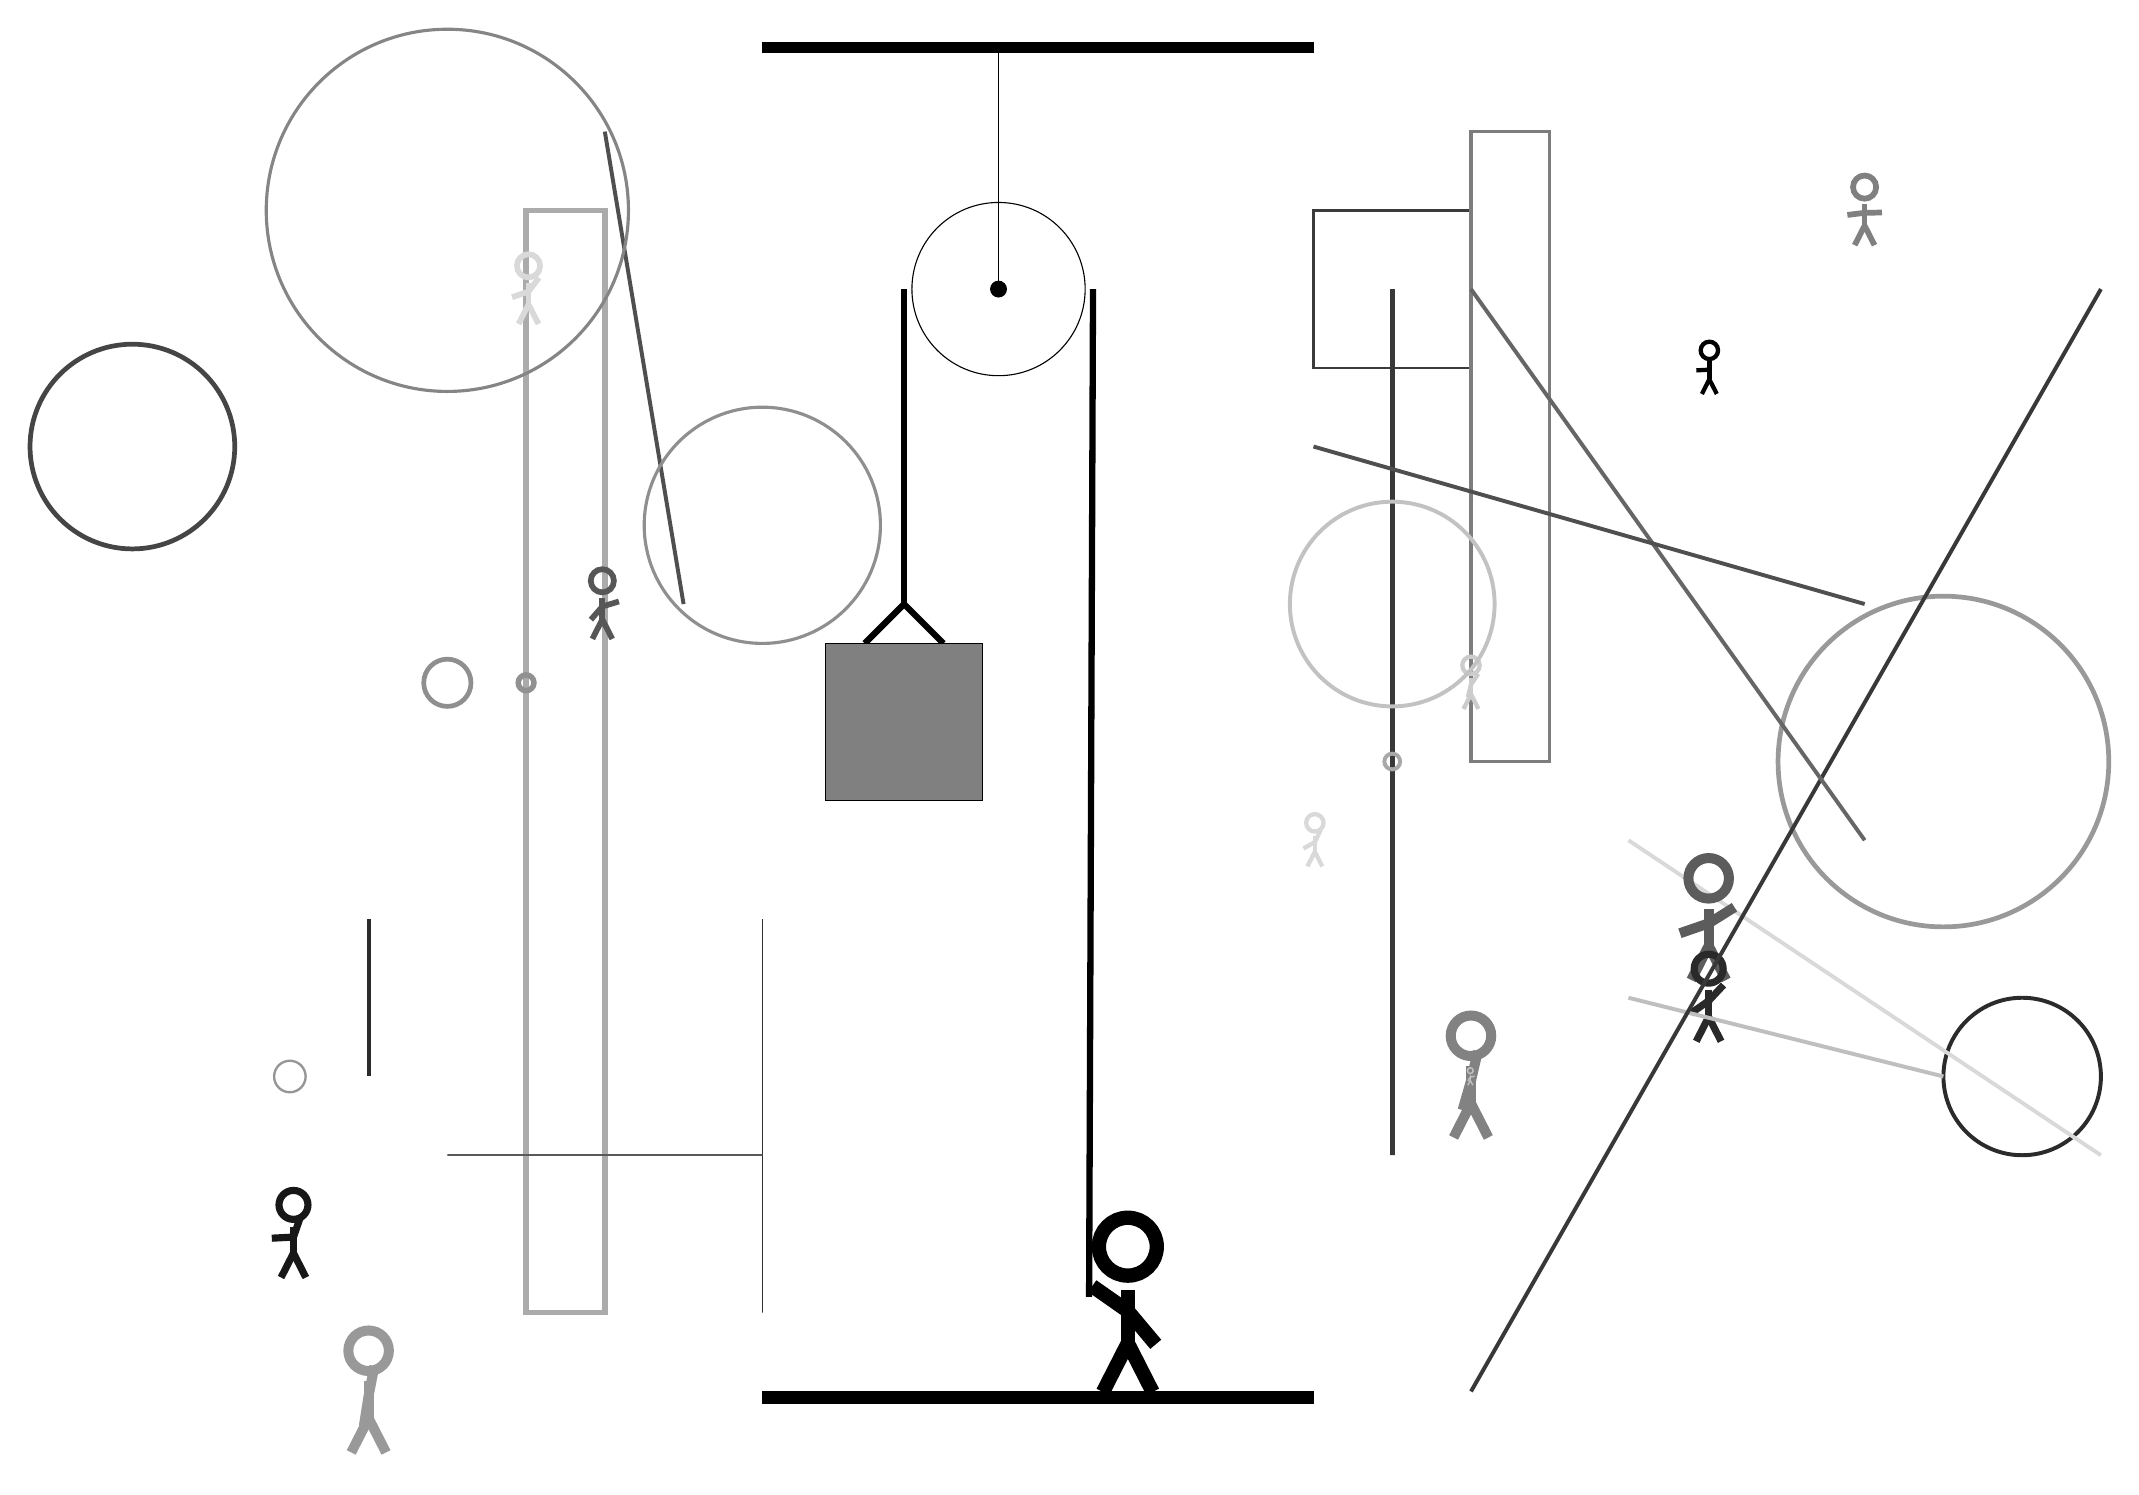
\begin{tikzpicture}
			%%%%% START %%%%%
			
			\draw[fill=black] (-2, 14) rectangle (5, 14.125);
			
			\draw (1, 11) circle (1.1);
			\draw[fill=black] (1, 11) circle (0.1);
			\draw (1, 14) -- (1, 11);
			
			\draw[line width=0.8mm] (-0.7, 6.5) -- (-0.2, 7.0) -- (0.3, 6.5);
			\draw[fill=black!50] (-1.2, 6.5) rectangle (0.8, 4.5);
			
			\draw[line width=0.8mm] (-0.2, 11) -- (-0.2, 7.0);
			\centerarc[line width=0.8mm](1, 11)(0:180:1.2000000000000002);
			\draw[line width=0.8mm](2.2, 11) -- (2.15, -1.8);
			
			\node[line width=0.2mm, color=black!100] at (10, 10) {\Strichmaxerl[3][3][90]};
			
			\draw[line width=0.3mm, color=black!77] (7, 12) rectangle (5, 10);
			\draw[line width=0.6mm, color=black!78] (6, 11) rectangle (6, 0);
			\draw [line width=0.5mm, color=black!83](14, 1) circle (1.0);
			\draw[line width=0.7mm, color=black!33] (-4, -2) rectangle (-5, 12);
			\node[line width=0.7mm, color=black!50] at (12, 12) {\Strichmaxerl[4][7][1]};
			\draw [line width=0.3mm, color=black!41](-8, 1) circle (0.2);
			\draw [line width=0.6mm, color=black!44](-6, 6) circle (0.3);
			\draw [line width=0.6mm, color=black!73](-10, 9) circle (1.3);
			\draw[line width=0.2mm, color=black!81] (-2, 3) rectangle (-2, -2);
			\node[line width=0.2mm, color=black!66] at (-4, 7) {\Strichmaxerl[4][49][17]};
			
			\draw[line width=0.4mm, color=black!51] (7, 13) rectangle (8, 5);
			\node[line width=0.5mm, color=black!20] at (7, 6) {\Strichmaxerl[3][76][56]};
			\node[line width=0.7mm, color=black!15] at (-5, 11) {\Strichmaxerl[4][19][53]};
			\draw [line width=0.6mm, color=black!40](13, 5) circle (2.1);
			\draw[line width=0.5mm, color=black!69](-3, 7) -- (-4, 13);
			
			\draw[line width=0.5mm, color=black!15](9, 4) -- (15, 0);
			\draw[line width=0.5mm, color=black!83](-7, 3) -- (-7, 1);
			\node[line width=0.6mm, color=black!64] at (10, 3) {\Strichmaxerl[7][19][32]};
			\node[line width=0.2mm, color=black!40] at (-7, -3) {\Strichmaxerl[7][81][79]};
			\node[line width=0.5mm, color=black!84] at (10, 2) {\Strichmaxerl[5][35][47]};
			\node[line width=0.5mm, color=black!49] at (7, 1) {\Strichmaxerl[7][74][77]};
			
			\draw[line width=0.5mm, color=black!25](9, 2) -- (13, 1);
			\draw[line width=0.2mm, color=black!65] (-2, 0) rectangle (-6, 0);
			\draw [line width=0.6mm, color=black!95](12, -2) circle (0.0);
			
			\node[line width=0.7mm, color=black!91] at (-8, -1) {\Strichmaxerl[5][3][71]};
			\draw[line width=0.5mm, color=black!78](7, -3) -- (15, 11);
			\draw [line width=0.5mm, color=black!34](6, 5) circle (0.1);
			
			\node[line width=0.5mm, color=black!15] at (5, 4) {\Strichmaxerl[3][29][64]};
			\draw[line width=0.5mm, color=black!60](7, 11) -- (12, 4);
			\draw [line width=0.4mm, color=black!44](-2, 8) circle (1.5);
			
			\node[line width=0.7mm, color=black!24] at (7, 1) {\Strichmaxerl[1][57][13]};
			\draw [line width=0.4mm, color=black!48](-6, 12) circle (2.3);
			\draw[line width=0.5mm, color=black!69](5, 9) -- (12, 7);
			\draw [line width=0.7mm, color=black!43](-5, 6) circle (0.1);
			\draw [line width=0.5mm, color=black!24](6, 7) circle (1.3);
			
			\node at (2.6, -1.9) {\Strichmaxerl[10][-35][-50]};
			
			\draw[fill=black] (-2, -3) rectangle (5, -3.15);
			
			%%%%% END %%%%%
		\end{tikzpicture}
	\end{figure}	
\end{document}